\chapter{Fundamentação}\label{fundamentacao}

Neste capítulo abordaremos como funcionam os principais tipos de CAPTCHA conhecidos, dando um enfoque especial aos CAPTCHAs baseados em texto. Em seguida, redes neurais são introduzidas como um problema de minimização e as técnicas de treino utilizadas neste trabalho são descritas.


\section{CAPTCHAS}

CAPTCHAs\cite{captcha2003} ou HIP (do inglês Human Interaction Proofs), são um conjunto de técnicas que tem como objetivo discernir a ação automatizada de robôs da ação de serem humanos na Rede Mundial de Computadores. Esses filtros tem sido usados de forma efetiva em diversas aplicações: proteger informações sensíveis, como \textit{e-mail} e dados pessoais; impedir tentativas de \textit{login} automatizados; acesso massivo a sistemas de bases de dados entre outros. Entretanto, desde as primeiras aplicações até os dias de hoje, existe uma corrida co-evolucionária entre atacantes e defensores. Por um lado, algoritmos de '\textit{quebra}' de CAPTCHA se  tornam cada vez mais sofisticados e precisos. Por outro lado, filtros mais complexos são desenvolvidos. Entretanto, como explicado por \cite{lectures2005HIP}, existe um balanço entre complexidade e factibilidade que os defensores devem buscar, explorando habilidades em que humanos ainda não foram ultrapassados por máquinas.

De forma geral, esses filtros podem ser formulados como um desafio sobre um conjunto de domínio cuja a resposta é um token. O domínio pode ser um trecho de áudio, uma sequencia de imagens ou até mesmo o histórico de navegação do desafiado. O token pode ser constituído de um conjunto de ações, o texto extraído de um áudio ou imagem, ou possuir um histórico de navegação confiável. Podem ainda ser constituídos de uma única etapa ou de varias. Na figura \ref{diffcaptchas} podemos ver diferentes tipos de CAPTCHAs gerados com a biblioteca de código aberto \textit{Securimage} \cite{securimage}.

\begin{figure}[ht]
	\begin{subfigure}{.5\textwidth}
		\centering
		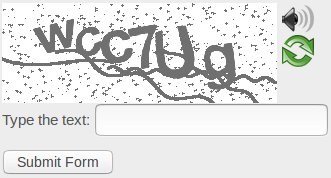
\includegraphics[width=.9\linewidth]{figuras/captcha_letras.png}
		\caption{Letras}
	\end{subfigure}
	\begin{subfigure}{.5\textwidth}
		\centering
		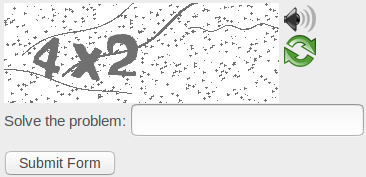
\includegraphics[width=.9\linewidth]{figuras/captcha_mat.png}
		\caption{Desafio matemático}
	\end{subfigure}%
	\vspace{.05\linewidth}
	\begin{subfigure}{.5\textwidth}
		\centering
		
\includegraphics[width=.9\linewidth]{figuras/captcha_texto.png}
		\caption{Duas palavras}
	\end{subfigure}
	\begin{subfigure}{.5\textwidth}
		\centering
		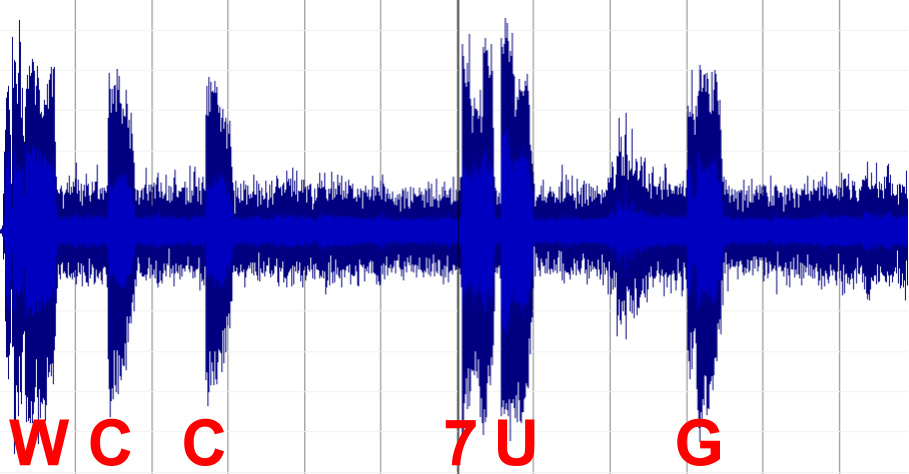
\includegraphics[width=.9\linewidth]{figuras/captcha_audio2.png}
		\caption{Áudio}
	\end{subfigure}
	\caption{Diferentes tipos de CAPTCHAs. (a) O desafiante deve reconhecer corretamente um texto formado por caracteres não correlacionados. (b) O desafiado deve resolver um problema simples de álgebra. (c) Palavras sorteadas de um repositório. (d) Reconhecimento de áudio. Gerados com a biblioteca Securimage.}
	\label{diffcaptchas}
\end{figure}

No subconjunto de CAPTCHAs baseados em texto, uma imagem contendo uma sequência de caracteres é exibida ao desafiado. O teste consiste em conseguir recuperar corretamente o texto codificado na imagem. Quanto ao texto, diferentes complexidades podem ser adicionadas: variar em tamanho, de alguns poucos a vários caracteres; ser composto por mais de uma palavra; utilizar diferentes alfabetos, apenas números, alfa-numérico, símbolos, diferenciar maiúsculas de minúsculas etc.; utilizar diferentes fontes, inclusive objetos que se assemelham à letras ou formas geométricas. Os caracteres podem ser sorteados aleatoriamente de forma independente a partir de um alfabeto ou serem oriundos de um repositório de palavras. Neste último caso, o desafio se torna mais fácil para humanos, dada nossa característica em reconhecer padrões, mas pode representar uma fraqueza caso a base seja exposta. Quanto à imagem, usualmente se utiliza adição de ruído, linhas e/ou grades para dificultar o processo de segmentação de caracteres \cite{lectures2005HIP}, efeitos de distorção como corrosão ou dilatação, transformações geométricas como rotação e translação, entre outros.  

Um exemplo da co-evolução desses sistemas é a forma como o reCaptcha \cite{recaptcha1} tem mudado ao longo dos anos. Quando proposto, o sistema era baseado em trechos de livros e jornais antigos que haviam falhado em processos de  OCR (do inglês optical character recognition). Trechos que não haviam sido corretamente identificados (teste) eram separados e exibidos para humanos juntamente com imagens cuja a extração era reconhecida (controle). Teste e controle eram comparados para certificar a atuação humana. Quando proposto, os autores alegaram que humanos eram capazes de resolver o desafio em quase todos os casos e que comutadores teriam chance quase nula de passarem desapercebidos, já que o repositório de exemplos era composta por imagens em que os melhores algoritmos haviam falhado. Porém, poucos anos depois, avanços em OCR obtiveram $99\%$ de precisão na base de texto utilizada por esse sistema \cite{captcha_break_2013}, inviabilizando o uso dessa técnica e forçando o reCaptcha a evoluir para uma segunda versão. Nessa nova abordagem, os dados de navegação dos usuários são analisados por um algoritmo de risco. Caso uma pontuação mínima seja atingida, o usuário é considerado humano, caso contrário, é exposto a problemas conhecidamente difíceis para computadores, como reconhecimento de objetos, contextualização de imagens e busca de similaridades, combinados com diferentes ações que devem ser performadas pelo usuário. Entretanto, mesmo essa nova versão pôde ser enganada por robôs em $85\%$ das vezes \cite{imarobot}, forçando a constante atualização dos desafios.

Em geral, o processo de '\textit{quebra}' envolve duas ideias principais: explorar vulnerabilidades ou uso de algoritmos inteligentes. Por serem testes automatizados, CAPTCHAs geralmente apresentam algum padrão de comportamento ou falha de projeto. A padronização na geração de desafios pode permitir que um atacante desenvolva heurísticas de ataque. Imagens com mesmo espaçamento de caracteres ou padrões repetitivos podem ser explorados e facilitar a segmentação da imagem, como foi explorado por \cite{naivecaptcha}, por exemplo. Falhas ou vieses no projeto de algoritmos também podem expor brechas. Nas primeiras versões do reCaptcha, por exemplo, possuir dados de navegação antigos era um dos principais critérios de avaliação de risco. De fato, essa foi a brecha explorada por \cite{imarobot} para conseguir uma alta taxa de sucesso. Quanto ao uso de algoritmos inteligentes, redes neurais recebem um lugar de destaque devido a flexibilidade e capacidade de generalização que esses modelos conseguem alcançar. O uso dessa classe de algoritmos foi a abordagem escolhida por \cite{captcha_break_2013} e \cite{lectures2005HIP}, por exemplo. Redes neurais são exploradas na sequência.


\section{Redes Neurais} \label{sec:neurais}

Dentro do campo de Inteligência Artificial, aprendizado de máquina é uma abordagem algoritmica para inferir regras em um problema a partir de exemplos. Uma categoria especial é a de aprendizado supervisionado, onde os exemplos constituem-se de um \textit{elemento} em um domínio conhecido e um \textit{rótulo} associado. O objetivo é deduzir abstrações que permitam relacionar elementos e rótulos. Nesse contexto, uma rede neural\footnote{Apesar de introduzidas aqui como um algoritmo supervisionado, redes neurais podem ser aplicadas de forma efetiva à problemas não supervisionados.} é, em última análise, uma forma genérica de escrever funções\footnote{Funções estão sendo usadas aqui com um sentido mais relaxado do que o usualmente utilizado na matemática.} sobre relações elementos-rótulos, transformando o desafio de encontrar regras em um problema de minimização, dado uma métrica de qualidade para as relações derivadas. O adjetivo '\textit{neural}' adivem da inspiração em funções biológicas que historicamente inspiraram e ainda inspiram essa forma de exprimir relações.

De forma mais específica, dado um conjunto de exemplos $D = \{(x, y)\}$, onde $x$  pertence ao domínio conhecido e $y$ um rótulo associado, desejamos encontrar a função $\hat{y} = f(x)$, de tal modo que $\hat{y}$ seja o mais similar possível à $y$. Por '\textit{mais similar o possível}' entende-se que conhecemos uma função de erro, também referida como função custo, que é tão menor quanto melhor for a aproximação dada por $f(x)$, e é normalmente representada como $J(y, \hat{y})$. Formalmente, desejamos encontrar $f^*$ tal que
\begin{equation}
f^* = \min_f J^{(D)} = \langle J(y, \hat{y}) \rangle_{D},
\end{equation}   
onde $\langle \ldots \rangle_{D}$ representa o valor esperado no conjunto $D$.

Redes neurais são um conjunto de técnicas inspiradas em processos cognitivos desempenhados pelo sistema nervoso que fornecem uma maneira de descrever famílias de funções. Dada uma família de funções $f^{\Theta} : x \rightarrow y$ definida por uma rede neural e parametrizadas por $\Theta$, podemos vasculhar o espaço de busca induzido por $\{\Theta\}$ para encontrar um função que satisfaça alguma propriedade de interesse. Em particular, no caso de aprendizado de máquina, estamos interessados em encontrar o parâmetro $\Theta^*$ tal que:
\begin{equation}
\Theta^* = \min_{\Theta} \langle J(y, f^{\Theta}(x)) \rangle_{D}.
\end{equation} 

Podemos utilizar composição de funções para construir redes neurais mais complexas e expressivas:
\begin{equation}
f^{\Theta}(x) = f^{\Theta_1}(f^{\Theta_2} (f^{\Theta_3}(\ldots(x))) ),
\end{equation}
sendo $\Theta = (\Theta_1, \Theta_2, \Theta_3, \ldots)$.
Quando compomos funções desta forma, é comum nos referirmos à cada função $f^{\Theta_i}$ como sendo a $i$-\textit{ésima} \textit{camada} da rede neural, sendo as camadas para além da mais externa também conhecidas como \textit{camadas escondias}. A \textit{profundidade} da rede é uma referência à quantidade de funções internas usadas na composição. Diferentes tipos de funções definem diferentes tipos de transformações, as quais nos referimos como tipo da camada. A especificação de todas as camadas em uma rede neural é o que chamamos de \textit{arquitetura} da rede. A seguir vamos explorar dois tipos de camadas que foram utilizados no presente estudo.

\subsection{Camadas Densas}

Camadas \textit{densas} ou totalmente conectadas definem uma transformação afim entre o conjunto de entradas e saídas. Tipicamente, após a transformação afim, segue-se a aplicação de uma função não linear elemento-à-elemento, conhecida como \textit{função de ativação}, permitindo a expressão de relações mais complexas entre esses dois conjuntos. As camadas densas são biologicamente inspiradas no mecanismo de comunicação dos neurônios, onde a diferença de potencial elétrico experimentado nos axônios é proporcional, em alguma medida, à soma das diferenças de potenciais nos dendritos.

De maneira mais formal, seja $x$ um vetor no conjunto de entrada, a relação expressa por uma camada densa é dada por:
\begin{equation}
f^{W,b}(x) = act(W \odot x + b)
\end{equation}
onde $b$ é um vetor, referido como \textit{viés}, $W$ uma matriz de transformação, $act$ uma função de ativação e $\odot$ é a operação usual de multiplicação de matrizes, definida elemento-à-elemento como $[W \odot x]_{i} = \sum_k W_{ik} * x_k$. Diferentes funções de ativação expressam diferentes não linearidades. Dentre os exemplos mais conhecidos na literatura, ressaltamos a função sigmoide $\sigma(z)_i = \frac{1}{1+\exp(-z_i)}$, que mapeia os elementos de saída no intervalo $\Re[0,1]$, a função de retificação linear (relu), definida por $relu(z)_i = max(0, z_i)$, e a função softmax, $\sigma(z)_i = \frac{\exp(z_i)}{\sum_j \exp(z_j)}$, que possui a interessante propriedade $\sum_i \sigma(z)_i = 1$, sendo usualmente utilizada para expressar distribuições de probabilidade.


\subsection{Camadas Convolucionais}

Camadas \textit{convolucionais} 


\begin{equation}
f^{W,b}(x) = act(W \otimes x + b)
\end{equation}

\begin{equation}
[W \otimes x]_{ijd} = \sum_{m=i'-k_i, n=j'-k_j}^{i'+ k_i, j'+k_j} W_{m, n, c, d} * x_{m, n, c}
\end{equation}
onde $k_i$ e $k_j$ são o tamanho do núcleo da transformação e a relação entre $s_i = i'/i$ ($s_j = j'/j$) definem o passo da transformação (em geral, $k_i = k_j = k$ e $s_i = s_j = s$). $W$ é um tensor de ranque 4 e $b$ um \textit{offset} com dimensão igual à última dimensão de $W$.

O núcleo da transformação define um campo perceptivo

\section{Aprendizado e Normalização}

Gradiente Descente, Rprop, Adam

Dropout, L2, L1, Batch-Norm



